Testing software is an integral part of the software development life cycle. It is necessary to guarantee that the product satisfies the design standards, as well as the expectations of the users. Identifying defects and performance issues before the product is delivered to the end user is its primary responsibility. This helps to ensure that the product's functionality and user pleasure are not compromised. By locating and enabling the correction of problems at an earlier stage in the development process, efficient software testing contributes to the enhancement of product quality. This, in turn, assists in the reduction of development costs while simultaneously enhancing reliability and performance. \cite{whatIsSoftwareTesting1}

In general, testing can be broken down into two categories: manual and automated approaches. Human testers are responsible for completing manual testing, which involves putting the program through a variety of activities and making a note of any faults or problems that occur. In spite of the fact that it has the potential to be very efficient in identifying particular kinds of faults, it tends to be more time-consuming and less dependable due to the presence of human error. When compared to manual testing, automated testing makes use of software tools to perform tests in a repetitive manner, which results in increased efficiency and consistency. The use of these tools allows for the rapid execution of thousands of complicated test cases during each test run, which provides coverage that is not attainable through the use of manual tests. \cite{whatIsSoftwareTesting2}

Part of the manual testing was experimenting with several \textbf{demo use-cases}, that are available in MP4 format, included in the annexes inside the demo folder.

\noindent\textbf{Testing the API Endpoints}

When it comes to API development, Postman is a vital tool that makes it easier to do both manual and automated testing by imitating the requests and responses of other users. It provides a user-friendly interface for submitting requests, showing and assessing results, and automating tests to evaluate various scenarios and performance outcomes. In addition, it allows users to send queries. Through the use of Postman, developers are able to effortlessly design and manage complete test suites that can systematically validate the functionality of API methods. \cite{postman}

API endpoints were subjected to thorough testing by means of a manual process that consisted of two primary methods. Initially, Postman was used to test the endpoints to ensure that they were able to function independently. Following a successful validation with Postman, additional testing was carried out using a web application that was developed based on these API endpoints. Because the functionality of the web application was heavily dependent on the robustness and reliability of the API endpoints, this second phase of testing was extremely important. 

It is also worth noting that the mobile application relies on the API for data retrieval, and possibly more in the future stages of development.

\noindent\textbf{Testing the Web Application}

The web application needed to be tested to confirm several feature aspects. The testing was done manually because automating the tests would have been beyond the scope of a developer. The process checked the authentication and authorization system to prevent unauthorized access to restricted resources. Verifying that the router component managed role-based resource access was also crucial. To ensure functionality and user satisfaction, the UI was tested. Testing also focused on smooth communication and data retrieval between the application and API to support the web application's functionality. This thorough testing strategy found and fixed issues, improving application reliability and security.

\noindent\textbf{Unit and Integration Testing}

Moq, a tool for mocking dependencies and external services, is essential for testing. Moq is a .NET mocking library that is used to isolate parts of the software being tested. It allows developers to create mock objects and configure their behavior, facilitating component testing independent of dependencies. \cite{moq}

I used Moq to mock application parts and dependencies, which helped me test the logic behind API and mobile app modules and components. This method made integration and unit testing easier, allowing for thorough application functionality testing. The following figure (\ref{fig:testcoverage}) shows that these tests covered my code well, proving their efficacy. This coverage demonstrates the tests' thoroughness and the testing methodology's reliability.

\begin{figure}[H]
	\centering
	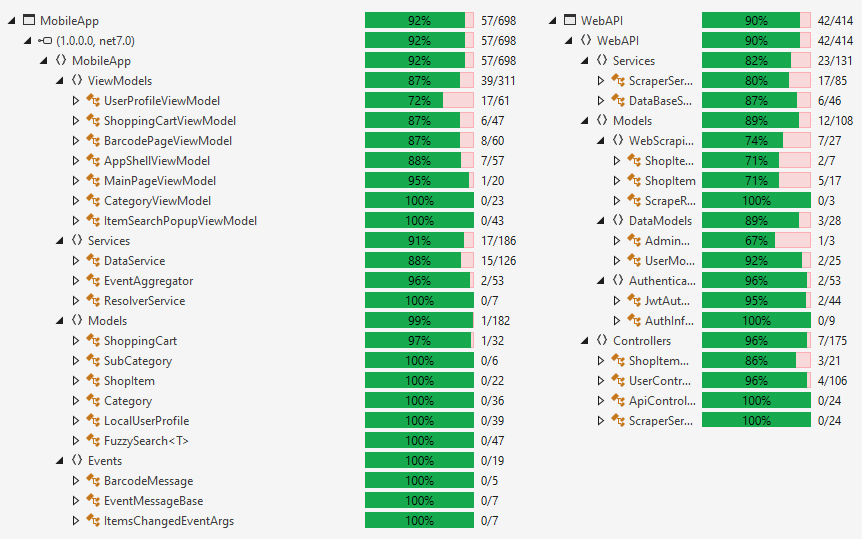
\includegraphics[width=0.8\linewidth]{img/testcoverage.png}
	\caption{Test Coverage Report}
	\label{fig:testcoverage}
\end{figure}